\documentclass[twoside,twocolumn]{article}

\usepackage{blindtext} % Package to generate dummy text throughout this template 
\usepackage{graphicx}
\usepackage[sc]{mathpazo} % Use the Palatino font
\usepackage[T1]{fontenc} % Use 8-bit encoding that has 256 glyphs
\linespread{1.05} % Line spacing - Palatino needs more space between lines
\usepackage{microtype} % Slightly tweak font spacing for aesthetics

\usepackage[english]{babel} % Language hyphenation and typographical rules

\usepackage[hmarginratio=1:1,top=32mm,columnsep=20pt]{geometry} % Document margins
\usepackage[hang, small,labelfont=bf,up,textfont=it,up]{caption} % Custom captions under/above floats in tables or figures
\usepackage{booktabs} % Horizontal rules in tables

\usepackage{lettrine} % The lettrine is the first enlarged letter at the beginning of the text

\usepackage{enumitem} % Customized lists
\setlist[itemize]{noitemsep} % Make itemize lists more compact

\usepackage{abstract} % Allows abstract customization
\renewcommand{\abstractnamefont}{\normalfont\bfseries} % Set the "Abstract" text to bold
\renewcommand{\abstracttextfont}{\normalfont\small\itshape} % Set the abstract itself to small italic text

\usepackage{titlesec} % Allows customization of titles
\renewcommand\thesection{\Roman{section}} % Roman numerals for the sections
\renewcommand\thesubsection{\roman{subsection}} % roman numerals for subsections
\titleformat{\section}[block]{\large\scshape\centering}{\thesection.}{1em}{} % Change the look of the section titles
\titleformat{\subsection}[block]{\large}{\thesubsection.}{1em}{} % Change the look of the section titles

\usepackage{fancyhdr} % Headers and footers
\pagestyle{fancy} % All pages have headers and footers
\fancyhead{} % Blank out the default header
\fancyfoot{} % Blank out the default footer
\fancyhead[L]{Comparativa de Gestiores de BD NoSQL } % Custom header text
\fancyhead[R]{November 2020 } % Custom header text
\fancyfoot[RO,LE]{\thepage} % Custom footer text

\usepackage{titling} % Customizing the title section

\usepackage{hyperref} % For hyperlinks in the PDF

%----------------------------------------------------------------------------------------
%	TITLE SECTION
%----------------------------------------------------------------------------------------

\setlength{\droptitle}{-4\baselineskip} % Move the title up

\pretitle{\begin{center}\Huge\bfseries} % Article title formatting
\posttitle{\end{center}} % Article title closing formatting
\title{COMPARATIVA DE USABILIDAD Y CURVA DE APRENDIZAJE DE AL MENOS DOS HERRAMIENTAS DE GESTIÓN DE PRUEBAS} % Article title
\author{Arias, Cancino, Crispin, Gutierrez, Zuñiga} 
\date{\today} % Leave empty to omit a date
\renewcommand{\maketitlehookd}{%
\begin{abstract}
	\begin{center}
		\textbf{Resumen}
	\end{center}
	Automatizar el proceso desde cambiar el código fuente hasta enviar su aplicación al entorno de producción es un factor de éxito.
Pero, ¿cómo construir una canalización de implementación? En este artículo se compara dos enfoques diferentes: acciones de GitHub y AWS CodePipeline.
\\
	\begin{center}
		
		\textbf{Abstract}
	\end{center}
	Automating the process from changing source code to submitting your application to production is a success factor.
But how do you build a deployment pipeline? This article compares two different approaches: GitHub Actions and AWS CodePipeline.
	\\
\end{abstract}
}
%----------------------------------------------------------------------------------------

\begin{document}
% Print the title
\maketitle
\vspace*{5 in}
\section{Introducción}
GitHub ha alojado código fuente durante más de diez años. Además de eso, GitHub anunció su servicio de CI / CD llamado Acciones de GitHub al público en noviembre de 2019.
AWS empodera a los desarrolladores con su servicio de entrega continua CodePipeline desde julio de 2015. Aproximadamente un año después, AWS anunció un complemento esencial: CodeBuild. Cuando escribo sobre CodePipeline a continuación, siempre me refiero a una combinación de CodePipeline y CodeBuild. Entonces, para ser más precisos, el título de esta publicación de blog debería ser: Acciones de GitHub frente a CodePipeline y CodeBuild.
\\
\section{Desarrollo}
\textbf{AWS CodePipeline}
\\\\La plataforma en la nube de Amazon ofrece una serie de soluciones para CI / CD. Investigamos los principales.
AWS CodePipeline es un servicio de entrega continua, que consta de diferentes etapas. Las etapas son una unidad que puede utilizar para aislar un entorno y limitar los cambios en ese entorno. En cada etapa, puede ejecutar una o más acciones sobre artefactos. Estos artefactos son colecciones de datos para su aplicación, por ejemplo, código fuente, dependencias, archivos de definiciones, etc.
AWS CodePipeline casi siempre se utiliza con AWS CodeBuild, que es un servicio de integración continua que compila código fuente, ejecuta pruebas y crea paquetes de software listos para implementar.
\\\\
\textbf{Github Actions}
\\\\GitHub Actions es un servicio integrado en GitHub. Tiene un mercado abierto con más de 6000 acciones para mejorar su flujo de trabajo. Estas acciones son creadas por usuarios, así como por organizaciones de confianza, como AWS, Docker o GitHub. Los flujos de trabajo pueden activarse mediante varios eventos de GitHub, como una solicitud de inserción o extracción. Decidimos hacer una herramienta CI / CD para nuestro servidor Juicy con una canalización de acciones de GitHub. 
\\\\
\textbf{Github Actions}
\\\\Tanto GitHub Actions como AWS CodePipeline utilizan conceptos similares para proporcionar una canalización de implementación:
\begin{itemize}
    \item Gestión del flujo de trabajo: personalice el flujo de trabajo de implementación según sus necesidades organizando acciones en paralelo o en orden.
    \item Ejecución de trabajos aislados: utilice imágenes de contenedor personalizadas o preconstruidas para proporcionar un entorno aislado para ejecutar acciones (por ejemplo, un trabajo de construcción).
\end{itemize}
En resumen, los conceptos principales son similares, pero ¿cuáles son las diferencias?
\\
\begin{center}
	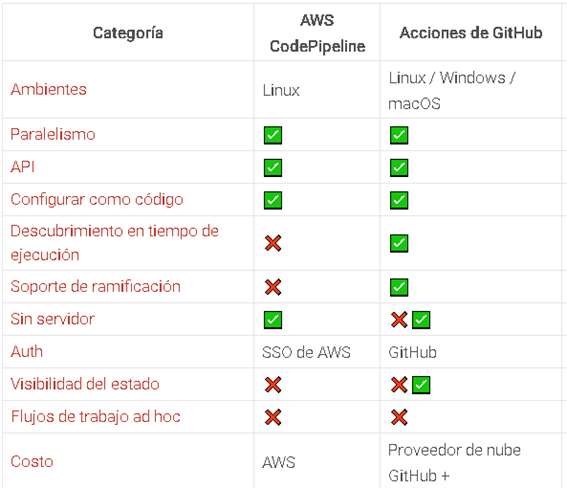
\includegraphics[ width=7cm]{./img/ga1.png} 
\end{center}
GitHub Actions ofrece una experiencia de desarrollador excepcional. Siempre que aloje su código fuente en GitHub, la solución es flexible, no solo por las integraciones (también conocidas como acciones) que se ofrecen en el mercado abierto. AWS CodePipeline se integra muy bien en el ecosistema de AWS. Poder utilizar roles de IAM para la autenticación en lugar de jugar con las claves de acceso para los usuarios de IAM es una gran ventaja.
\\\\
\textbf{Comparación}
\\\\Decidir cuál es la mejor solución para su situación depende de muchas cosas. Puede haber muchas razones y consideraciones diferentes para elegir entre las soluciones de AWS en comparación con las acciones de GitHub. Pero para nosotros, por ahora, los factores más importantes fueron:
\begin{itemize}
    \item Ambas soluciones tienen un precio por minuto de construcción. Además, AWS cobra un costo fijo mensual por canalización. La ventaja de las acciones de GitHub aquí es que se define una cantidad máxima de minutos, por lo que los costos finales son más fáciles de predecir.
    \item Repositorio de código fuente. Acciones de GitHub solo admite GitHub como repositorio de código fuente, mientras que AWS CodePipeline también admite Bitbucket, AWS CodeCommit y Amazon S3.
    \item Como se mencionó anteriormente, GitHub Actions funciona con un mercado abierto. Estos varían en calidad, ya que está abierto a publicar para todos. En comparación, AWS tiene sus propias integraciones de alta calidad.
    \item Autenticación de AWS. La gran ventaja de CodePipeline es que la autenticación se maneja con roles de IAM en lugar de claves de acceso para los usuarios de IAM. Con las acciones de GitHub, debe almacenar las claves de acceso del usuario de IAM en secretos de GitHub.
    \item Las acciones de GitHub son muy fáciles de usar, mientras que CodePipeline es más difícil de comenzar. CodePipeline será más valioso tan pronto como lo integre con otros servicios de Amazon (por ejemplo, CodeBuild, CodeDeploy y más).
\end{itemize}
\textbf{Instalación}
\\\\La instalación de una herramienta de construcción puede ser el primer obstáculo a superar.\\\\
Si está en AWS, la herramienta más fácil de "instalar" es AWS CodePipeline, ya que no hay instalación. Es un servicio de primera clase que proporciona AWS. Siempre que tenga permisos para acceder al servicio, puede comenzar a construir una canalización.\\\\
La experiencia de instalación de Acciones de GitHub estará determinada por su tipo de cuenta y lo que desea lograr. Si está ejecutando un proyecto de código abierto, entonces no hay instalación. Está incluido en el repositorio. Si necesita ejecutar las acciones en su propia infraestructura, deberá instalar algunos corredores . La forma en que lo haga dependerá probablemente de las herramientas que ya utilice. El equipo en el que trabajo actualmente ha configurado la infraestructura con AWS Cloud Developer Kit (CDK) y los agentes con Ansible . Esto significa que tenemos un flujo de trabajo repetible para escalar a los finalistas, si es necesario.
\\\\
\textbf{Ambientes}
\\\\Comprender en qué entornos necesita ejecutar las compilaciones puede ayudarlo a determinar qué herramienta es la adecuada para usted. Si desea utilizar la misma herramienta de compilación en todos los proyectos que compilan para Windows, Linux y macOS, eso limitaría la elección de la herramienta. Puede decidir elegir una herramienta que se adapte a una plataforma o unir muchas herramientas.
\\\\
\textbf{Paralelismo}
\\\\Antes de que se dé cuenta, hablará sobre los tiempos de construcción y cómo puede reducirlos. Una de las formas más fáciles de lograr esto es ejecutar pasos / tareas en paralelo.\\\\
Esto es posible dentro de AWS CodePipeline, pero ahí es donde se detiene la ejecución paralela. No puede ejecutar muchos pasos dentro de la etapa de AWS CodeBuild. Por ejemplo, supongamos que tiene una etapa de análisis estático dentro de la canalización. Tal vez ejecute un linter, un verificador de seguridad y un verificador de estilo de código. Es probable que esté en un buildspec.ymlarchivo y deberá ejecutarlos de forma secuencial.\\\\
En Acciones de GitHub puede ejecutar una construcción de matriz , que es similar. En su archivo de flujo de trabajo, puede definir una estrategia de matriz para la ejecución del trabajo. Actualmente, esto solo se puede hacer a nivel de flujo de trabajo. Esto es útil, por ejemplo, si desea verificar que su compilación y pruebas funcionan en muchas versiones de un idioma. No ayuda con el escenario de análisis estático mencionado anteriormente. Sin embargo, en Acciones de GitHub podrías definir un flujo de trabajo por herramienta, que a su vez lo convertiría en ejecución paralela. Tenga en cuenta, sin embargo, que significaría que está gastando más dinero en el corredor de acción (dependiendo del plan de precios en el que se encuentre). Esto se debe a que tendría que clonar el repositorio, instalar todas las dependencias, etc. muchas veces, cada una de las cuales incurre en "costos de tiempo de ejecución".
\\\\
\textbf{Configurar como código}
\\\\Este ha sido un artículo bastante caro en la industria durante muchos años. Esta es la idea de que la configuración de recursos debe administrarse como código fuente en su repositorio. Hay demasiado de qué hablar sobre este tema, así que lo dejaremos ahí para esta publicación.\\\\
Todas las herramientas se adaptan a esto. Para ver en qué se diferencian, consulte el capítulo siguiente, que cubre las ligeras diferencias en su enfoque.
\\\\
\textbf{Descubrimiento en tiempo de ejecución}
\\\\Esta sección trata esencialmente sobre el mantenimiento. ¿Puede la herramienta “descubrir” lo que necesita ser ejecutado por el código y la configuración dentro de la rama y la base de código?\\\\
AWS CodePipeline debe tener definida una canalización estática. Cada etapa se define en algo como CDK / Terraform o manualmente. Esto luego se puede delegar en un buildspec.ymlarchivo dentro del repositorio, pero la canalización en sí es estática. Esto significa que si su canalización necesita cambiar ligeramente entre las ramas, debe implementar los cambios estáticos.\\\\
Acciones de GitHub descubre el flujo de trabajo, por rama y ejecuta lo que encuentra en el archivo de flujo de trabajo. Esto es deseable, ya que todo está dentro de la base de código / rama / solicitud de extracción. No hay ninguna configuración oculta.
\\\\
\textbf{Soporte de ramificación}
\\\\Esto solo se menciona realmente, debido a una limitación dentro de AWS CodePipeline, en este momento. En este momento, una CodePipeline se puede vincular a una rama de git.\\\\
Debido a esto, significa que necesitará administrar muchas canalizaciones para cubrir algunas estrategias de ramificación, por ejemplo, GitFlow . Esto es una sobrecarga para su equipo, así que tenga esto en cuenta.\\\\
Las acciones de GitHub tienen una sintaxis "[on]" que le permite definir patrones para que coincidan. También puede ejecutar sentencias if dentro del flujo de trabajo para proteger ciertos pasos según la rama.
\\\\
\textbf{Sin servidor}
\\\\AWS CodePipline y AWS CodeBuild se proporcionan como una función sin servidor dentro de AWS. Es decir, no se le pedirá que cuide ningún servidor. Siempre que defina sus pipelines, ya sea manualmente o como código, el resto será cuidado por usted.\\\\
Las acciones de GitHub son similares, a menos que desee ejecutar agentes en sus propios servidores. Si lo hace, entonces necesita administrar esa pieza de infraestructura.
\\\\
\textbf{Auth}
\\\\La autenticación y autorización para AWS CodePipline y GitHub Actions están cubiertas por el acceso normal a esa herramienta.\\\\
Para AWS CodePipeline, las personas que necesitan interactuar con una canalización necesitarán acceso de IAM a las cuentas que ejecutan las canalizaciones. Esto puede ser deseable o no.\\\\
Esto es similar para las acciones de GitHub, pero le permite restringir el acceso a ciertos repositorios dentro de su organización.
\\\\
\textbf{Visibilidad del estado}
\\\\Ha elegido una herramienta y ahora tiene muchos trabajos definidos, que cubren muchos repositorios y proyectos. Poder ver, de un vistazo, el estado de tus proyectos es clave. Quieres comentarios rápidos y prácticos.\\\\
AWS CodePipeline ha mostrado recientemente la ejecución más reciente de una canalización en la pantalla de canalizaciones.
\begin{center}
	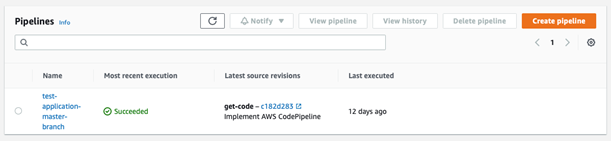
\includegraphics[ width=7.5cm]{./img/ga2.png} 
\end{center}
Esta es una adición muy necesaria. Esto proporciona una descripción general de todas sus canalizaciones en la cuenta de región a la que está accediendo. Vale la pena señalar que todos los miembros de su equipo, o cualquier persona que necesite ver estos datos, necesitarán acceder a su cuenta de AWS, lo que puede no ser ideal. La sugerencia aquí sería crear roles de IAM para bloquear esto, pero esto viene con una sobrecarga.\\\\
Acciones de GitHub es una pestaña en el repositorio. Actualmente, no puede obtener una vista, dentro de GitHub, que le muestre el estado en muchos repositorios para un proyecto determinado.\\\\
Muestra claramente cada ejecución para cada rama dentro del repositorio.
\begin{center}
	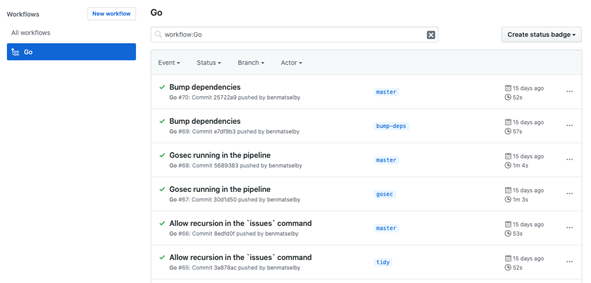
\includegraphics[ width=7.5cm]{./img/ga3.png} 
\end{center}
\textbf{Flujos de trabajo ad hoc}
\\\\Si estás en un equipo al que le gusta automatizar muchas cosas, entonces esa automatización tendrá que ejecutarse en alguna parte. Un lugar obvio parece ser tu herramienta de construcción.\\\\
AWS CodePipeline y GitHub Actions no sirven para trabajos ad hoc. AWS CodePipeline necesita un activador y luego ejecuta una canalización estática. Acciones de GitHub está escuchando eventos de git.
\\\\
\textbf{Costo}
\\\\AWS CodePipline se cobra dentro del modo de precios de AWS. Sin embargo, como se mencionó anteriormente, también necesitará el servicio AWS CodeBuild, que también es de pago .\\\\
Las acciones de GitHub se cobran a las organizaciones. Si necesita ejecutar agentes en sus servidores, incurrirá en costos de infraestructura.

\section{Conclusiones}
Durante este articulo, configuramos dos canalizaciones, una con cada proveedor. Esto nos dio mucha información sobre las posibilidades y limitaciones de cada solución.

\section{Biblografia}

\begin{itemize}
    \item https://medium.com/@karthickcse05/aws-code-pipeline-vs-github-actions-8643b31165ce
    \item https://docs.github.com/en/free-pro-team@latest/github/setting-up-and-managing-billing-and-payments-on-github/about-billing-for-github-actions
    \item https://cloudonaut.io/github-actions-vs-aws-codepipeline/
    \item https://benmatselby.dev/post/build-tool-comparison/
\end{itemize}

%%%%%%%%%%%%%%%%%%%%%%%%%%%%%%%%%%%%%%%%%%%%%%%%%%%%%%%%%
\end{document}